\def\SigleNumero{STT-1900}
\def\NomCours{Méthodes statistiques pour l'ingénierie}
\def\DateEvaluation{17 octobre 2025}
\def\HeureEvaluation{18h30 à 20h20}
\def\Session{}
\def\NomEvaluation{Examen 1}
\def\Ponderation{35}
% Ne rien mettre entre les accolades si l'enseignant (ou l'enseignante) est aussi le coordonnateur (ou la coordonnatrice)
\def\Coordonnatrice{}
\def\Coordonnateur{}

% Ne rien mettre entre les accolades s'il y a plus d'une section
\def\Enseignant{}
\def\Enseignante{}

% Ne rien mettre entre les accolades s'il s'agit d'un cours à section unique
% Mettre le nom de chacun des enseignants et enseignantes entre les accolades
% Une case à cocher sera générée pour chacune des sections
\def\SectionA{Thierry Duchesne (section à distance)}
\def\SectionB{Julien Miron (section en classe)}
\def\SectionC{}
\def\SectionD{}


\def\Directives{
\begin{enumerate}
\item Matériel autorisé:
\begin{itemize}
    \item Calculatrice scientifique {\bf autorisée par la faculté des sciences et de génie};
    \item Une seule feuille aide-mémoire \textbf{manuscrite} de format lettre (8.5''$\times$11'') recto-verso;
    \item Les tables de lois distribuées avec cet examen. S'il-vous-plaît, ne rien écrire sur celles-ci.
    \end{itemize}
\item Assurez-vous que cette évaluation comporte \numquestions ~questions réparties sur \numpages{}~pages, pour un total de \numpoints{}~points.\
\item \textbf{Veuillez ne pas dégrafer votre examen.}
\item Ajoutez vos initiales dans le bas de chaque page (sauf pour les tables de lois).
\item Vous devez\textbf{ justifier toutes vos réponses} par une démarche claire, sauf pour les questions à choix de réponse.\
\item Pour les questions à choix de réponse et les vrais ou faux, vous pouvez mettre un X, un crochet ($\checkmark$) ou remplir la case.\
\item Certains vrais ou faux demandent une justification. Aucun point ne sera donné sans justification, même si vous cochez la bonne réponse.
\item Pour les questions à choix de réponse, lorsqu'il est écrit «cochez tous les énoncés qui sont vrais/faux», il est possible qu'un seul énoncé soit vrai.
\item Le verso des feuilles peut être utilisé comme brouillon, \textbf{mais ne sera pas corrigé}. Attention à ne rien dégrafer.
\end{enumerate}
}



\documentclass{Evaluation}
\usepackage{multicol,graphicx}
\begin{document}

\pageblanche
%%%%%%%%%%%%%%%% QUESTION %%%%%%%%%%%%%%%%
\begin{questions}


\question[6]\label{module1_1}  
On nous donne les probabilités suivantes:
\[
\begin{aligned}
    & P(A) = 0,45 \\
    & P(B) = 0,25 \\
    & P(C) = 0,30 \\
    & P(C|A) = 0,30 \\
    & P(C|B) = 0,30 \\
    & P(A \cap B) = 0,05 \\
\end{aligned}
\]

Cochez tous les énoncés qui sont \textbf{vrais}, sachant que trois énoncés sont vrais. \textit{Chaque énoncé qui est coché alors qu'il ne devrait pas l'être annule les points d'un élément coché qui devrait l'être.}
\begin{checkboxes}
\correctchoice La probabilité de l'événement complémentaire de \(A\) est $ P(\overline{A}) = 0,55 $
\correctchoice $ P(A \cap \overline{B}) = 0,40 $
\choice $ P(A \cup C) = 0,75 $
\correctchoice $A$ et $C$ sont indépendants
\choice Comme $B$ et $C$ sont indépendants, ils sont mutuellement exclusifs
\end{checkboxes}



\vspace{0.5cm}
\question[3] Lequel des énoncés suivants est vrai?

\begin{checkboxes}
    \choice Pour pouvoir utiliser le théorème central limite, il faut que les variables aléatoires soient normales et que $n\geq 30$.
    \correctchoice Une combinaison linéaire de variables aléatoires normales indépendantes suit \textbf{toujours} une loi normale.
    \choice Si $X\sim\mathcal{N}(\mu,\sigma^2)$, pour calculer $P(X=3)$, il suffit de calculer la fonction de densité évaluée en $x=3$.
    \choice Si $X_1,\hdots,X_8$ sont des réalisations d'une loi normale d'espérance $\mu$ et de variance $\sigma^2$, nous ne pouvons pas dire que $\overline{X}$ suit une loi normale d'espérance $\mu$ et de variance $\sigma^2/n$, car $n=8<30$.
\end{checkboxes}


\pageblanche

% développement proba cond

\question On vous dit que 20 \% des nouvelles publiées sur un réseau social sont publiées par des trolls (T), 50 \% sont publiées par de véritables journalistes (V)
et 30 \% sont publiées par des intelligences artificielles (I). Une étude démontre que 3/4 des nouvelles publiées par les trolls sont fausses, alors que
la proportion de fausses nouvelles est de 1/10 chez les véritables journalistes et de 2/3 pour les intelligences artificielles. 
Utilisez F pour dénoter l'événement <<la nouvelle est fausse>>.

    \begin{parts}
    \part[6] Quelle proportion des nouvelles publiées sur ce réseau social sont fausses ?

    \begin{solution}
    On a $P(T)=0,20$, $P(V)=0,50$, $P(I)=0,30$, $P(F|T)=3/4$, $P(F|V)=1/10$, $P(F|I)=2/3$ et on cherche $P(F)$.
    Puisque $\{T,V,I\}$ forment une partition de l'espace échantillonnal, on peut utiliser la loi des probabilités totales :
    \begin{align*}
        P(F) &= P(F|T)P(T)+P(F|V)P(V)+P(F|I)P(I) 
        = \frac{3}{4}\times 0,20+\frac{1}{10}\times 0,50 + \frac{2}{3}\times 0,30\\
        &= \frac{8}{20} =\frac{4}{10}=\frac{2}{5}=0,40.
    \end{align*}
    \end{solution}

    \vspace{8 cm}

    \part[6]  Une nouvelle que vous trouvez particulièrement choquante est publiée sur ce réseau, mais vous ignorez par qui/quoi. Il s'avère que cette nouvelle n'est PAS fausse. Quelle est
    la probabilité qu'elle ait été publiée par une intelligence artificielle ?

    \begin{solution}
    On cherche $P(I|\bar{F})$. On peut utiliser la règle de Bayes :
    \begin{align*}
        P(I|\bar{F}) &= \frac{P(\bar{F}|I)P(I)}{P(\bar{F})} =\frac{\{1-P({F}|I)\}P(I)}{1-P({F})} \\
        &= \frac{\{1-2/3\}(3/10)}{1-0,40}=\frac{1}{6}\approx 0,1667.
    \end{align*}
    \end{solution}

    \end{parts}

\pageblanche

% normale en 2 parties, une seule normale et une combinaison linéaire de normales

\question Soit $X$, le volume d'eau qui arrive dans un bassin dans une journée. Soit $Y$, le volume d'eau puisée de ce même bassin dans une journée. 
Les volumes d'eau sont en milliers de mètres cubes. 
On vous dit que $X$ et $Y$ sont des variables aléatoires indépendantes qui suivent toutes deux des lois normales, avec 
$X\sim \mathcal{N}(8,4)$ et $Y\sim \mathcal{N}(12,9)$.

    \begin{parts}
    \part[5] On souhaite redimensionner le bassin de sorte que son nouveau volume devra être égal au $0,985^{\text{e}}$ quantile de la distribution de la quantité d'eau y arrivant dans une journée. Quel devra être ce nouveau volume ?

\begin{solution}
    On cherche $v$ tel que 
    \begin{align*}
           P[N(8,4)\le v]=0,985\Leftrightarrow P\left[N(0,1)\le\frac{v-8}{\sqrt{4}} \right]=0,985\\
           \Rightarrow \frac{v-8}{2}=2,17 \Rightarrow v=12,34,
    \end{align*}
    autrement dit le nouveau volume doit être de 12~340 mètres cubes.
\end{solution}

    \vspace{8 cm}

    \part[7]  Dans une journée donnée, quelle est la probabilité que la quantité d'eau puisée du bassin soit supérieure au double de la quantité d'eau qui arrive dans le bassin ?

    \begin{solution}
        On cherche $P(X_P>2X_A)$ :
        \begin{align*}
            P(X_P>2X_A) &= P(2X_A-X_P<0)\ \ \ \ \ \ [{\text{ou}}\ P(X_P-2X_A>0)] \\
             &= P\left[N\left\{2(8)-12,~2^2(4)+(-1)^29\right\}<0\right]=P\left[N\left\{4,~25\right\}<0\right]\\
             &= P\left[N(0,1)<\frac{0-4}{\sqrt{25}}\right]=\Phi(-0,8)=1-\Phi(0,8)=1-0,78814\\
             &=0,21186.
        \end{align*}
    \end{solution}

    \end{parts}



\pageblanche

% normale et TCL 

\question[10] Vous vendez 100 véhicules. Pour chacun, le prix inclut 2 000 \$ pour couvrir les frais de garantie; au total, vous avez donc 200 000 \$ de provision.
Soit $C_1,\dots,C_{100}$ les coûts que vous devez rembourser aux clients pour des problèmes sous garantie pour chacun de ces 100 véhicules vendus. 

On vous dit que
$C_1,\dots,C_{100}$ est un échantillon aléatoire d'une loi inconnue d'espérance 1~950~\$ et d'écart-type 400~\$. Quelle est la probabilité approximative
que la provision ne soit pas suffisante pour couvrir les coûts de la garantie ? Autrement dit, calculez la valeur approximative de
$$P\left(\sum_{i=1}^{100}C_i > 200~000\right).$$

\begin{solution}
\begin{align*}
    P\left(\sum_{i=1}^{100}C_i > 200~000\right) &= P\left(\frac{\sum_{i=1}^{100}C_i}{100} > \frac{200~000}{100}\right)
=P\left(\frac{\bar{C}-1~950}{400/\sqrt{100}} > \frac{2~000-1~950}{400/\sqrt{100}}\right)\\
 &\approx P\left(N(0,1) > \frac{50}{40}\right)=1-\Phi(1,25)=1-0,89435=0,10565.
\end{align*}  
\end{solution}



\pageblanche

% mais ça fait un beau lien avec les notes de cours. en fait c'est un premier jet pour poser l'idée, on pourra tenter d'améliorer
% mais j'aimerais autre chose que toujours la normale

\question\label{EQM} La quantité de pluie (en mm) tombée dans un bassin versant
dans un mois suit une loi ayant comme fonction de répartition
$$F(x)=\left\{\begin{array}{ll}
0, & x<0\\
1-e^{-x/\theta}, & x\ge 0,
\end{array}\right.$$
où $\theta>0$ est un paramètre de valeur inconnue. On peut montrer que $E(X)=\theta$ et $V(X)=\theta^2$.

La compagnie qui gère un barrage à la sortie de ce bassin versant a besoin de savoir l'espérance et la variance de la quantité de pluie tombée
dans un mois afin d'optimiser la gestion du barrage. L'ingénieure de la compagnie a à sa disposition un échantillon aléatoire $X_1,\dots,X_{20}$
provenant de cette loi, dont elle souhaite se servir pour estimer les quantités désirées. Soit $\displaystyle \overline{X}=\frac{1}{20}\sum_{i=1}^{20}X_i$.

\vspace{0.25cm}
    \begin{parts}
    \part[5] Calculez l'espérance de $\overline{X}$. Est-ce que $\overline{X}$ est un estimateur sans biais de $\theta$ ? 



    \begin{solution}
        $E(\bar{X})=E(X_i)=\theta$, et donc oui, $\bar{X}$ est un estimateur sans biais de $\theta$
    \end{solution}


    \vspace{7 cm}
    \part[6]  Calculez l'espérance de $\overline{X}^2$. Est-ce que $\overline{X}^2$ est un estimateur sans biais de $\theta^2$ ?
    
    [Aide :\ Souvenez-vous que pour toute variable aléatoire $Y$,\ \ $V(Y)=E(Y^2)-\{E(Y)\}^2$.\ \ \ \ ]

    \begin{solution}
        $$E(\bar{X}^2)=V(\bar{X})+\{E(\bar{X})\}^2=\frac{\theta^2}{20}+\{\theta\}^2=\frac{21}{20}\theta^2
        \neq\theta^2\Rightarrow\text{Non, $\bar{X}^2$ n'est pas sans biais pour $\theta^2$.}$$
    \end{solution}


    \end{parts}

  \pageblanche  
\question Soit l'histogramme suivant:

\begin{center}
    
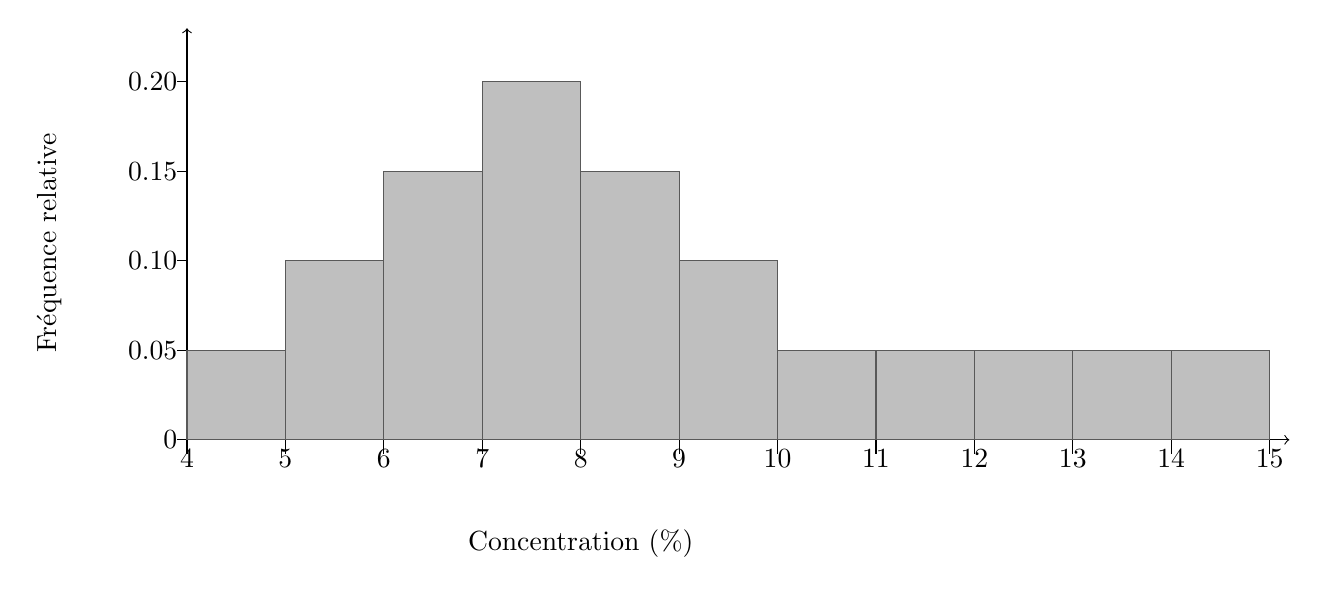
\begin{tikzpicture}[x=1.25cm, y=22.727cm] % 10 cm de large (8 unités) et 5 cm de haut (0.22 unités)
  % Axes
  \draw[->] (4,0) -- (15.2,0);
  \draw[->] (4,0) -- (4,0.23);

  % Graduations en x
  \foreach \x in {4,...,15} {
    \draw (\x,0) -- (\x,-0.008);
    \node[below] at (\x,0) {\x};
  }

  % Graduations en y
  \foreach \y/\lab in {0/0,0.05/0.05,0.10/0.10,0.15/0.15,0.20/0.20}{
    \draw (4,\y) -- (3.9,\y);
    \node[left] at (4,\y) {\lab};
  }

  % Titres d'axes
  \node[below] at (8,-0.045) {Concentration (\%)};
  \node[rotate=90] at (2.6,0.11) {Fréquence relative};

  % Barres : classes [4,5[, [5,6[, ..., [11,12[
  \foreach \x/\h in {4/0.05,5/0.1,6/0.15,7/0.20,8/0.15,9/0.1,10/0.05,11/0.05,12/0.05,13/0.05,14/0.05} {
    \fill[gray!50] (\x,0) rectangle (\x+1,\h);
    \draw[gray!70!black] (\x,0) rectangle (\x+1,\h);
  }
\end{tikzpicture}
\end{center}

Déterminez si les énoncés suivants sont vrais ou faux. 

\textbf{\textit{Une bonne réponse vaut 2 points, une mauvaise réponse vaut -1 point et une réponse vide vaut 0 point, pour un total minimum de 0 point.}}

\vspace{0.5cm}
\begin{parts}
    \part[2] Il est impossible de donner la taille de l'échantillon qui a servi à tracer cet histogramme avec l'information donnée.

    \begin{oneparcheckboxes}
        \correctchoice Vrai
        \choice Faux
    \end{oneparcheckboxes}

\vspace{0.25cm}
\part[2] Cet histogramme est typique de données provenant d'une distribution où la moyenne est supérieure à la médiane.

    \begin{oneparcheckboxes}
        \correctchoice Vrai
        \choice Faux
    \end{oneparcheckboxes}

\vspace{0.25cm}
\part[2] L'écart interquartile vaut au moins 5,5.

    \begin{oneparcheckboxes}
        \choice Vrai
        \correctchoice Faux
    \end{oneparcheckboxes}

    \vspace{0.25cm}

\part[2] La médiane échantillonnale est entre 7\% et 9\%, inclusivement.

    \begin{oneparcheckboxes}
        \correctchoice Vrai
        \choice Faux
    \end{oneparcheckboxes}

\part[2] L'écart-type échantillonnal est de 11\%.

    \begin{oneparcheckboxes}
        \choice Vrai
        \correctchoice Faux
    \end{oneparcheckboxes}
    
    \end{parts}


    

    \pageblanche
    \question Soit $X_1,\hdots,X_{25}$, des réalisations indépendantes d'une variable aléatoire normale d'espérance $\mu=176,45$ et d'écart-type $\sigma=\sqrt{48}$.

    \begin{parts}
        \part[6] Quelle est la probabilité que la variance échantillonnale soit supérieure à 46,68?
\begin{solution}
    \begin{align*}
        P(S^2>46,68)&=P(\frac{24S^2}{48}>23,34)\\
        &=P(U>23,34)\, \, \text{où $U\sim\chi^2_{24}$}\\
        &=0,5
    \end{align*}
\end{solution}
        \vspace{10cm}

        \part[6] Quelle est la probabilité que la moyenne échantillonale soit supérieure à $\mu+0,749 ~ S$, où $S$ est l'écart-type échantillonnal ?
    \begin{solution}
    \begin{align*}
        P(\overline{X}>\mu+0,69S)&=P(\overline{X}-\mu>0,69S)\\
        &=P(\frac{\overline{X}-\mu}{S}>0,69)\\
        &=P(\frac{\overline{X}-\mu}{S/\sqrt{5}}>3,45)\\
        &=P(T>3,45)\, \, \text{où $T\sim t_{25}$}\\
        &= 0,001
    \end{align*}
\end{solution}
    \end{parts}
    
    \pageblanche
    

\question\label{repartition} Soit la variable aléatoire $X$ dont la fonction de répartition est donnée par:

$$F(x)=\left\{\begin{array}{ll}
0, & x<0,\\
x^2, & 0\leq x \leq 1,\\
1, & x>1.
\end{array}\right.$$
\begin{parts}

    \part[4] Quelle est la valeur de la médiane de $X$?

\begin{solution}
    On cherche $m$ tel que $P(X<m)=0,5$ (ou plus grand). Comme on a la fonction de répartion, on trouve directement 
    \begin{align*}
        F(m)&=0,5\\
        m^2&=0,5\\
        m&=\sqrt{0,5}
    \end{align*}
On garde seulement la valeur positive, car $X$ est définie sur l'intervalle $[0,1]$.
\end{solution}
    \vspace{7cm}
    \part[6] Calculez la probabilité que $X$ soit compris entre 0,2 et 0,3, sachant que $X$ est supérieur à 0,1.

\begin{solution}
    \begin{align*}
        P(0,2<X<0,3|X>0,1)&=\frac{P(0,2<X<0,3 \cap X>0,1)}{P(X>0,1)}\\
        &=\frac{P(0,2<X<0,3)}{P(X>0,1)}\\
        &=\frac{F(0,3)-F(0,2)}{1-F(0,1)}\\
        &=\frac{0,3^2-0,2^2}{1-0,1^2}\\
        &=\frac{0,05}{0,99}\\
        &=\frac{5}{99}
    \end{align*}
\end{solution}
\vfill
    \pagesuivante{\ref{repartition}}
\pageblanche
\suite{\ref{repartition}}

    \part[4] Donnez la fonction de densité de $X$.

    \begin{solution}
$$f(x)=\left\{\begin{array}{ll}
\frac{d}{dx}0, & x<0,\\
\frac{d}{dx}x^2, & 0\leq x \leq 1,\\
\frac{d}{dx}1, & x>1.
\end{array}\right.$$

$$f(x)=\left\{\begin{array}{ll}
2x, & 0\leq x \leq 1,\\
0, & \text{sinon}.
\end{array}\right.$$
    \end{solution}
\end{parts}
\pageblanche

\question On souhaite obtenir un intervalle de confiance pour $\mu$, l'espérance d'une variable aléatoire $X$ normale de variance $0,81$, à l'aide de l'échantillon suivant:

$$1,1,1,2,2,2,3,3,3,$$
pour lequel $\displaystyle\sum_{i=1}^n x_i=18$ et $\displaystyle\sum_{i=1}^9x_i^2=42$.

\begin{parts}
    \part[5] Donnez l'intervalle de confiance de niveau $95\%$.

    \begin{solution}
        Il s'agit d'un intervalle de confiance pour $\mu$, cas loi normale variance connue, donc l'IC est de la forme
        $$\overline{X}\pm z_{\alpha/2}\frac{\sigma}{\sqrt{n}}$$
        Ici, $\overline{x}=2$, $\alpha/2=0,025$, donc $z_{\alpha/2}=1,96$, $\sigma=\sqrt{0,81}$ et $\sqrt{n}=3$.

        L'intervalle de confiance est donc
        \begin{align*}
            [2-1,96\frac{0,9}{3}&;2=1,96\frac{0,9}{3}]\\
            [1,412&;2,588]
        \end{align*}
    \end{solution}
    \vspace{10cm}

    \part[5] Quel devrait-être le niveau de l'intervalle de confiance pour qu'il soi t de longueur 0,708?

    \begin{solution}
        Si l'intervalle de confiance est de longueur 0,708, cela implique que la marge d'erreur est de longueur $0,708/2=0,354$.

        Donc 
        \begin{align*}
            z_{\alpha/2}\frac{\sigma}{\sqrt{n}}&=0,354\\
            z_{\alpha/2}\frac{0,9}{3}&=0,354\\
            z_{\alpha/2}&=1,18
        \end{align*}
        
    \end{solution}
\end{parts}
\pageblanche
\end{questions}

\end{document} 
